\section{Memory Banks}

  \begin{definition}[Memory]
    The \textbf{memory} is where the computer stores data and instructions, which can be though of as a giant array of memory addresses, with each containing a byte. This data consists of graphical things or even instructions to manipulate other data. It can be visualized  as a long array of boxes that each have an \textbf{address} (where it is located) and \textbf{contents} (what is stored in it).

    Memory simply works as a bunch of bits in your computer with each bit having some memory address, which is also a bit. For example, the memory address \texttt{0b0010} (2) may have the bit value of \texttt{0b1} (1) stored in it. 

    \begin{figure}[H]
      \centering 
      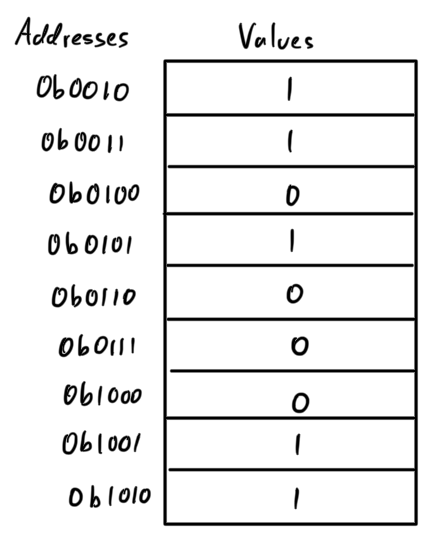
\includegraphics[scale=0.4]{img/memory_visual_bit.png}
      \caption{Visualization of memory as a long array of boxes of bits. }
      \label{fig:memory_visual_bit}
    \end{figure}

    However, computers do not need this fine grained level of control on the memory, and they really work at the Byte level rather than the bit level. Therefore, we can visualize the memory as a long array of boxes indexed by \textit{Bytes}, with each value being a byte as well. In short, the memory is \textbf{byte-addressable}. In certain arthitectures, some systems are \textbf{word-addressable}, meaning that the memory is addressed by words, which are 4 bytes.\footnote{Note that in here the size of a word is 2 bytes rather than 4 as stated above. This is just how it is defined in some \texttt{x86} architectures.}

    \begin{figure}[H]
      \centering 
      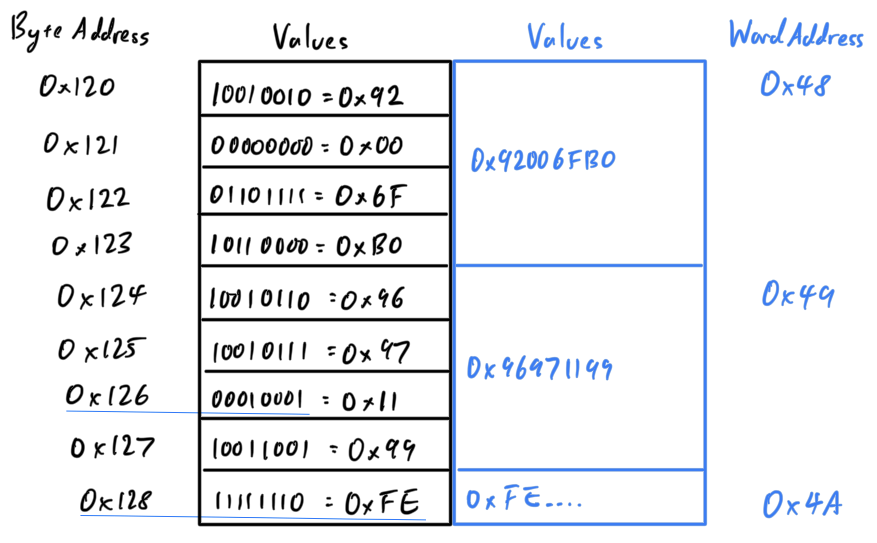
\includegraphics[scale=0.4]{img/memory_visual_byte.png}
      \caption{Visualization of memory as a long array of boxes of bytes. Every address is a byte and its corresponding value at that address is also a byte, though we represent it as a 2-digit hex. } 
      \label{fig:memory_visual_byte}
    \end{figure}
  \end{definition}

  It is intuitive to think that given some multi-byte object like an \texttt{int} (4 bytes), the beginning of the int would be the lowest address and the end of the int would be the highest address, like how consecutive integers are stored in an array. However, this is not always the case (almost always not the case since most computers are little-endian).  

  \begin{definition}[Endian Architecture]
    Depending on the machine architecture, computers may store these types slightly differently in their \textit{byte} order. Say that we have an integer of value \texttt{0xA1B2C3D4} (4 bytes). Then, 
    \begin{enumerate} 
      \item A \textbf{big-endian architecture} (e.g. SPARC, z/Architecture) will store it so that the least significant byte has the highest address.
      \item A \textbf{little-endian architecture} (e.g. x86, x86-64, RISC-V) will store it so that the least significant byte has the lowest address. 
      \item A \textbf{bi-endian architecture} (e.g. ARM, PowerPC) can specify the endianness as big or little. 
    \end{enumerate}

    \begin{figure}[H]
      \centering 
      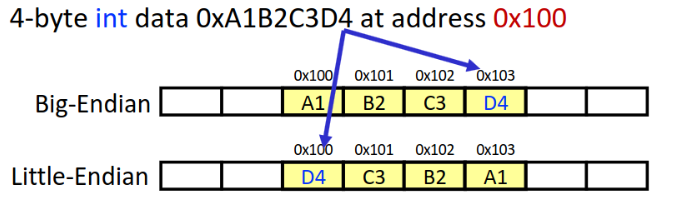
\includegraphics[scale=0.4]{img/endianness.png}
      \caption{The big vs little endian architectures. } 
      \label{fig:endianness}
    \end{figure}
  \end{definition}

  We can simply print out the hex values of primitive types to see how they are stored in memory, but it does not provide the level of details that we want on which bytes are stored where. At this point, we must use certain \textbf{debuggers} to directly look at the memory. For x86 architectures, we can use \texttt{gdb} and for ARM architectures, we can use \texttt{lldb}. At this point, we need to understand assembly to look through debuggers, so we will provide the example here. 

  To clarify, let us compare registers and memory. Memory is addressed by an unsigned integer while registers have names like \texttt{\%rsi}. Memory is much bigger at several GB, while the total register space is much smaller at around 128 bytes (may differ depending on the architecture). The memory is much slower than registers, which is usually on a sub-nanosecond timescale. The memory is dynamic and can grow as needed while the registers are static and cannot grow.

